%%%%%%%%%%%%%%%%%%%%%%%%%%%%%%%%%%%%%%%%%
% Beamer Presentation
% LaTeX Template
% Version 1.0 (10/11/12)
%
% This template has been downloaded from:
% http://www.LaTeXTemplates.com
%
% License:
% CC BY-NC-SA 3.0 (http://creativecommons.org/licenses/by-nc-sa/3.0/)
%
%%%%%%%%%%%%%%%%%%%%%%%%%%%%%%%%%%%%%%%%%

%----------------------------------------------------------------------------------------
%	PACKAGES AND THEMES
%----------------------------------------------------------------------------------------

\documentclass{beamer}

\mode<presentation> {

% The Beamer class comes with a number of default slide themes
% which change the colors and layouts of slides. Below this is a list
% of all the themes, uncomment each in turn to see what they look like.

%\usetheme{default}
%\usetheme{AnnArbor}
%\usetheme{Antibes}
%\usetheme{Bergen}
% \usetheme{Berkeley}
%\usetheme{Berlin}
%\usetheme{Boadilla}
\usetheme{CambridgeUS}
%\usetheme{Copenhagen}
% \usetheme{Darmstadt}
%\usetheme{Dresden}
% \usetheme{Frankfurt}
%\usetheme{Goettingen}
%\usetheme{Hannover}
%\usetheme{Ilmenau}
%\usetheme{JuanLesPins}
%\usetheme{Luebeck}
% \usetheme{Madrid}
%\usetheme{Malmoe}
%\usetheme{Marburg}
%\usetheme{Montpellier}
% \usetheme{PaloAlto}
%\usetheme{Pittsburgh}
%\usetheme{Rochester}
%\usetheme{Singapore}
%\usetheme{Szeged}
%\usetheme{Warsaw}

% As well as themes, the Beamer class has a number of color themes
% for any slide theme. Uncomment each of these in turn to see how it
% changes the colors of your current slide theme.

% \usecolortheme{albatross}
% \usecolortheme{beaver}
% \usecolortheme{beetle}
%\usecolortheme{crane}
\usecolortheme{dolphin}
%\usecolortheme{dove}
% \usecolortheme{fly}
%\usecolortheme{lily}
% \usecolortheme{orchid}
% \usecolortheme{rose}
% \usecolortheme{seagull}
% \usecolortheme{seahorse}
% \usecolortheme{whale}
% \usecolortheme{wolverine}

%\setbeamertemplate{footline} % To remove the footer line in all slides uncomment this line
%\setbeamertemplate{footline}[page number] % To replace the footer line in all slides with a simple slide count uncomment this line

%\setbeamertemplate{navigation symbols}{} % To remove the navigation symbols from the bottom of all slides uncomment this line
}

\usepackage{graphicx} % Allows including images
\usepackage{booktabs} % Allows the use of \toprule, \midrule and \bottomrule in tables
\usepackage{amsmath}
\usepackage{amsthm}
\usepackage{xcolor}
\usepackage{graphicx}
\usepackage{amsfonts}
\usepackage{amssymb}
\usepackage {tikz}
\usepackage{caption}
\usepackage{subcaption}
\usepackage{circuitikz}
\usepackage {xcolor}
\usepackage{wasysym}
\usepackage[lined,linesnumbered]{algorithm2e}
\usepackage{bibentry}
\usepackage{animate}

\usetikzlibrary{graphs,graphs.standard}
\setbeamercovered{transparent=8}
\usetikzlibrary{positioning}
\newcommand{\Mset}[2]{\ensuremath{\mathbb{M}_{#1 \times #2}}}
\newcommand{\reff}[1][e]{\ensuremath{R_#1^{\text{eff}}}}
\newcommand{\laplacian}[1][G]{\ensuremath{L_{#1}^{+}}}
\newcommand{\reffformula}[1][\laplacian]{\ensuremath{ (\chi_u - \chi_v)^T \  #1 \ (\chi_u - \chi_v) }}

\newcommand{\proj}{\ensuremath{I - \frac{\textbf{1} \textbf{1}^T}{n}}}
\newcommand{\sqlaplacian}[1][G]{\ensuremath{\sqrt{L_{#1}^{+}}}}
% \newcommand{\Mset}[2]{\ensuremath{\mathbb{M}_{#1 \times #2}}}
% \newcommand\norm[1]{\left\lVert#1\right\rVert}

% from https://tex.stackexchange.com/questions/107186/how-to-write-norm-which-adjusts-its-size
\newcommand\norm[1]{\left\lVert#1\right\rVert}

\usepackage{lipsum}

\newcommand\Fontvi{\fontsize{6}{7.2}\selectfont}
\newcommand{\Lim}[1]{\raisebox{0.5ex}{\scalebox{0.8}{$\displaystyle \lim_{#1}\;$}}}

% \shorthandoff{=}
%----------------------------------------------------------------------------------------
%	TITLE PAGE
%----------------------------------------------------------------------------------------

\title[Random Spanning Trees]{Random Spanning Trees} % The short title appears at the bottom of every slide, the full title is only on the title page

\author{Bhishmaraj S} % Your name
\institute[CMI] % Your institution as it will appear on the bottom of every slide, may be shorthand to save space
{
Chennai Mathematical Institute \\ % Your institution for the title page
\medskip
\textit{bhishma@cmi.ac.in} % Your email address
}
\date{\today} % Date, can be changed to a custom date

\begin{document}

\begin{frame}
\titlepage % Print the title page as the first slide
\end{frame}

\begin{frame}
\frametitle{Overview} % Table of contents slide, comment this block out to remove it

\tableofcontents % Throughout your presentation, if you choose to use \section{} and \subsection{} commands, these will automatically be printed on this slide as an overview of your presentation
\end{frame}

%----------------------------------------------------------------------------------------
%	PRESENTATION SLIDES
%----------------------------------------------------------------------------------------

%------------------------------------------------
\section{Introduction} % Sections can be created in order to organize your presentation into discrete blocks, all sections and subsections are automatically printed in the table of contents as an overview of the talk
%------------------------------------------------

\subsection{Problem Definition} % A subsection can be created just before a set of slides with a common theme to further break down your presentation into chunks

\begin{frame}
\frametitle{Problem Definition}
% \begin{block}

 Given an undirected connected graph $G = (V, E)$, sample a spanning tree $T$ with probability $\frac{1}{|\mathcal{T}|}$ where $\mathcal{T}$ denotes the set of all spanning trees of $G$. 
 
%  
% \end{block}

% \begin{block}

% \onslide<2->{

\end{frame}

\subsection{Applications}

\begin{frame}

\frametitle{Applications}
 
Sampling spanning trees pops up in surprising problems in TCS such as 

\begin{itemize}
\pause
\item Constructing expanders (\cite{10.5555/1496770.1496834}, \cite{doi:10.1137/120890971})
\pause
\item Approximation algorithms for TSP(\cite{6108216}, \cite{doi:10.1287/opre.2017.1603})
\pause
\item Graph Sparsification (\cite{DBLP:journals/corr/abs-1005-0265}, \cite{dolev2016random})
\pause
\item Analysis of network reliability (\cite{10.5555/535891},\cite{doi:10.1002/net.3230200303}, \cite{colbourn1988estimating})
\pause
\item Sequence shuffling problem in Bioinformatics (\cite{KANDEL1996171})

\end{itemize}

% \pause
\onslide<6->{
Maze Generation \footnote{\url{https://en.wikipedia.org/wiki/Maze_generation_algorithm}}

% \begin{figure}
% 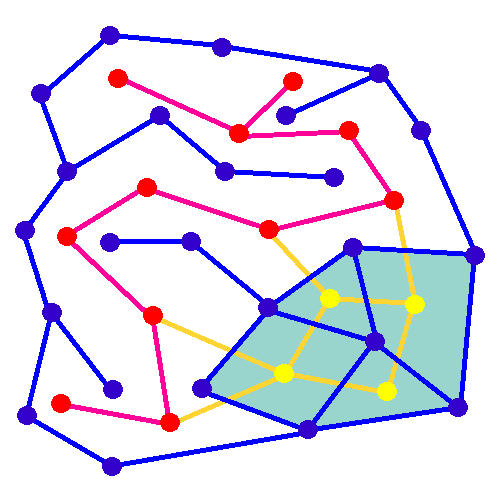
\includegraphics[scale=0.1]{gif_png/maze-11} 
% \end{figure}
}
%  \leavevmode\hphantom{ }
%   \leavevmode\hphantom{ }
% \pause


% \centering


% \pause
% \hspace*{\fill}
% \animategraphics[loop,controls,width=\linewidth,scale=0.2]{15}{gif_png/maze-}{0}{17}

% 
% }
% \end{block}



\end{frame}

%------------------------------------------------

\subsection{A bird's eye view of existing algorithms}
\begin{frame}
 \frametitle{Proposed Algorithms}
 
 In this talk we would review some of the algorithms proposed for this problem and get into details of \cite{harvey2016generating}  
 
 \leavevmode\hphantom{ }
 
 \begin{itemize}
 \pause
  \item \textbf{Random Walk Based} - Simulate variants of random walk on the input graph
  \pause
  \item \textbf{Determinant Based} - Based on Kirchoff Matrix Tree theorem and involve computing determinants of the laplacian matrix
  \pause
  \item  \textbf{Approximation Algorithms}
 \end{itemize}

 
 
\end{frame}

\section{Random Walk Based Algorithms}

\subsection{Aldous-Broder Algorithm}

\begin{frame}
\frametitle{Aldous-Broder Algorithm}

 Andrei Broder and David Aldous independently invented the following algorithm
 
 

\begin{figure}
% \centering
\scalebox{0.7}{
\begin{algorithm}[H]
 \KwIn{$G = (V,E)$}
 \KwOut{A random spanning tree}
 
 Choose a starting vertex $s$ arbitrarily
 
 $T_V \leftarrow \{s\}, T_E \leftarrow \emptyset$
 
 \While{$|T_V| < |V$} {
 
    $next =_{u.a.r} N(s)$
    
    \If{$next \not\in T_V$} {
        $T_V = T_V \cup \{next\}$
        
        $T_E = T_E \cup \{(s, next)\}$
    }
    
    $s = next$
 
 }
 
 \KwRet{$T = (T_V, T_E)$}

 
  \caption{Aldous-Broder Algorithm}
\end{algorithm}
 }
\end{figure} 
\end{frame}


\begin{frame}
\frametitle{Aldous-Broder Algorithm example}

\only<1>{
\begin{figure}
\centering
\begin {tikzpicture}[auto ,node distance =4 cm and 5cm ,on grid ,
semithick ,
state/.style ={ circle  , 
draw,black , text=black , minimum width =1 cm}]
\node[state] (C){$C$};
\node[state, fill=white!50!green] (A) [above =of C] {$A$};
\node[state] (B) [above right =of C] {$B$};
\node[state] (D) [right =of C] {$D$};
\path (C) edge[very thick] (D);
\path (B) edge[very thick] (D);
\path (A) edge[very thick] (B);
\path (C) edge[very thick] (A);
\path (D) edge[very thick] (A);
\end{tikzpicture}
 
\end{figure}
}

\only<2>{
\begin{figure}
\centering
\begin {tikzpicture}[auto ,node distance =4 cm and 5cm ,on grid ,
semithick ,
state/.style ={ circle  , 
draw,black , text=black , minimum width =1 cm}]
\node[state] (C){$C$};
\node[state, fill=white!50!red] (A) [above =of C] {$A$};
\node[state, fill=white!50!green] (B) [above right =of C] {$B$};
\node[state] (D) [right =of C] {$D$};
\path (C) edge[very thick] (D);
\path (B) edge[very thick] (D);
\path (A) edge[very thick,blue] (B);
\path (C) edge[very thick] (A);
\path (D) edge[very thick] (A);
\end{tikzpicture}
 
\end{figure}
}

\only<3>{
\begin{figure}
\centering
\begin {tikzpicture}[auto ,node distance =4 cm and 5cm ,on grid ,
semithick ,
state/.style ={ circle  , 
draw,black , text=black , minimum width =1 cm}]
\node[state] (C){$C$};
\node[state, fill=white!50!green] (A) [above =of C] {$A$};
\node[state, fill=white!50!red] (B) [above right =of C] {$B$};
\node[state] (D) [right =of C] {$D$};
\path (C) edge[very thick] (D);
\path (B) edge[very thick] (D);
\path (A) edge[very thick,blue] (B);
\path (C) edge[very thick] (A);
\path (D) edge[very thick] (A);
\end{tikzpicture}
 
\end{figure}
}

\only<4>{
\begin{figure}
\centering
\begin {tikzpicture}[auto ,node distance =4 cm and 5cm ,on grid ,
semithick ,
state/.style ={ circle  , 
draw,black , text=black , minimum width =1 cm}]
\node[state] (C){$C$};
\node[state, fill=white!50!red] (A) [above =of C] {$A$};
\node[state, fill=white!50!red] (B) [above right =of C] {$B$};
\node[state, fill=white!50!green] (D) [right =of C] {$D$};
\path (C) edge[very thick] (D);
\path (B) edge[very thick] (D);
\path (A) edge[very thick,blue] (B);
\path (C) edge[very thick] (A);
\path (D) edge[very thick, blue] (A);
\end{tikzpicture}
 
\end{figure}
}

\only<5>{
\begin{figure}
\centering
\begin {tikzpicture}[auto ,node distance =4 cm and 5cm ,on grid ,
semithick ,
state/.style ={ circle  , 
draw,black , text=black , minimum width =1 cm}]
\node[state] (C){$C$};
\node[state, fill=white!50!red] (A) [above =of C] {$A$};
\node[state, fill=white!50!green] (B) [above right =of C] {$B$};
\node[state, fill=white!50!red] (D) [right =of C] {$D$};
\path (C) edge[very thick] (D);
\path (B) edge[very thick] (D);
\path (A) edge[very thick,blue] (B);
\path (C) edge[very thick] (A);
\path (D) edge[very thick, blue] (A);
\end{tikzpicture}
 
\end{figure}
}

\only<6>{
\begin{figure}
\centering
\begin {tikzpicture}[auto ,node distance =4 cm and 5cm ,on grid ,
semithick ,
state/.style ={ circle  , 
draw,black , text=black , minimum width =1 cm}]
\node[state] (C){$C$};
\node[state, fill=white!50!red] (A) [above =of C] {$A$};
\node[state, fill=white!50!red] (B) [above right =of C] {$B$};
\node[state, fill=white!50!green] (D) [right =of C] {$D$};
\path (C) edge[very thick] (D);
\path (B) edge[very thick] (D);
\path (A) edge[very thick,blue] (B);
\path (C) edge[very thick] (A);
\path (D) edge[very thick, blue] (A);
\end{tikzpicture}
 
\end{figure}
}

\only<7>{
\begin{figure}
\centering
\begin {tikzpicture}[auto ,node distance =4 cm and 5cm ,on grid ,
semithick ,
state/.style ={ circle  , 
draw,black , text=black , minimum width =1 cm}]
\node[state, fill=white!50!green] (C){$C$};
\node[state, fill=white!50!red] (A) [above =of C] {$A$};
\node[state, fill=white!50!red] (B) [above right =of C] {$B$};
\node[state, fill=white!50!red] (D) [right =of C] {$D$};
\path (C) edge[very thick, blue] (D);
\path (B) edge[very thick] (D);
\path (A) edge[very thick,blue] (B);
\path (C) edge[very thick] (A);
\path (D) edge[very thick, blue] (A);
\end{tikzpicture}
 
\end{figure}
}


\end{frame}



\begin{frame}

\pause
\frametitle{Running Time}

\textbf{Cover Time}

$cov_G(u) := $ The expected number of steps for a random walk starting at $u$ to visit all the vertices in $G$

\leavevmode\hphantom{ }

\pause
\textbf{Cover Time of $G$} 

$cov_G := \max_{u \in V_G} cov_G(u)$ 

 \leavevmode\hphantom{ }
 
 \pause
 It is known that $cov_G = \mathcal{O}(|V|\ |E|) = \mathcal{O}(|V|^3)$

 

% \pause
% \centering
%  \begin{tikzpicture}
%   \graph { subgraph K_n [n=5,clockwise,radius=2cm] };
% \end{tikzpicture}

\end{frame}

\subsection{Wilson's Algorithm}

\begin{frame}
 \frametitle{Wilson's Algorithm}
 
 In 1996 Wilson proposed a variant of random walk called loop erased random walk .
\begin{figure}
\scalebox{0.7}{
\begin{algorithm}[H]

 \KwIn{$G = (V,E) \  \text{and} \  \text{root } r \in V$}
 \KwOut{Parent pointer array called $next$}

 $\text{inTree}[i] \leftarrow False, \; \forall \ i \neq r$
 
 $\text{inTree}[r] \leftarrow True$
 
 $\text{next}[r] \leftarrow \text{NULL}$
 
 \For{$i \leftarrow 1$ to $n$ }{
    
    $u = i$
    
    \While{$\neg \text{inTree}[u]$} {
    
        $\text{next}[u] =_{u.a.r} N(u)$
        
        $u = \text{next}[u]$
    
    }
    
    $u = i$
    
    \While{$\neg \text{inTree}[u]$} {
    
        $\text{inTree}[u] = True$
        
        $u = \text{next}[u]$
    
    }
    
    
 }
 \KwRet{next}
 
 \caption{Wilson's Algorithm}
 
\end{algorithm}
 
 }
 
\end{figure}

 
 
\end{frame}



\begin{frame}
 \frametitle{Wilson's algorithm example}
 
 \only<1>{
\begin{figure}
\centering
\begin {tikzpicture}[auto ,
semithick ,
state/.style ={ circle  , 
draw,black , text=black , minimum width =1 cm}]
\node[state] (A){$A$};
\node[state] (B) [above right=of A] {$B$};
\node[state] (C) [right =of B] {$C$};
\node[state] (D) [below right =of A] {$D$};
\node[state] (E) [right =of D] {$E$};
\node[state, fill=white!50!red] (F) [above right =of E] {$F$};

\path (C) edge[very thick] (D);
\path (B) edge[very thick] (D);
\path (A) edge[very thick] (B);
\path (C) edge[very thick] (B);
\path (D) edge[very thick] (A);
\path (D) edge[very thick] (E);
\path (C) edge[very thick] (E);
\path (C) edge[very thick] (F);
\path (F) edge[very thick] (E);
\end{tikzpicture}
 
\end{figure}
}
 
 \only<2>{
 
 Start at $A$ 
\begin{figure}
\centering
\begin {tikzpicture}[auto ,
semithick ,
state/.style ={ circle  , 
draw,black , text=black , minimum width =1 cm}]
\node[state, fill=white!50!green] (A){$A$};
\node[state] (B) [above right=of A] {$B$};
\node[state] (C) [right =of B] {$C$};
\node[state] (D) [below right =of A] {$D$};
\node[state] (E) [right =of D] {$E$};
\node[state, fill=white!50!red] (F) [above right =of E] {$F$};

\path (C) edge[very thick] (D);
\path (B) edge[very thick] (D);
\path (A) edge[very thick] (B);
\path (C) edge[very thick] (B);
\path (D) edge[very thick] (A);
\path (D) edge[very thick] (E);
\path (C) edge[very thick] (E);
\path (C) edge[very thick] (F);
\path (F) edge[very thick] (E);
\end{tikzpicture}
 
\end{figure}
}

 
 \only<3>{
\begin{figure}
\centering
\begin {tikzpicture}[auto ,
semithick ,
state/.style ={ circle  , 
draw,black , text=black , minimum width =1 cm}]
\node[state, fill=white!50!blue] (A){$A$};
\node[state, fill=white!50!green] (B) [above right=of A] {$B$};
\node[state] (C) [right =of B] {$C$};
\node[state] (D) [below right =of A] {$D$};
\node[state] (E) [right =of D] {$E$};
\node[state, fill=white!50!red] (F) [above right =of E] {$F$};

\path (C) edge[very thick] (D);
\path (B) edge[very thick] (D);
\path[->] (A) edge[very thick, blue]  (B);
\path (C) edge[very thick] (B);
\path (D) edge[very thick] (A);
\path (D) edge[very thick] (E);
\path (C) edge[very thick] (E);
\path (C) edge[very thick] (F);
\path (F) edge[very thick] (E);
\end{tikzpicture}
 
\end{figure}
}

 \only<4>{
\begin{figure}
\centering
\begin {tikzpicture}[auto ,
semithick ,
state/.style ={ circle  , 
draw,black , text=black , minimum width =1 cm}]
\node[state, fill=white!50!blue] (A){$A$};
\node[state, fill=white!50!blue] (B) [above right=of A] {$B$};
\node[state,fill=white!50!green] (C) [right =of B] {$C$};
\node[state] (D) [below right =of A] {$D$};
\node[state] (E) [right =of D] {$E$};
\node[state, fill=white!50!red] (F) [above right =of E] {$F$};

\path (C) edge[very thick] (D);
\path (B) edge[very thick] (D);
\path[->] (A) edge[very thick, blue]  (B);
\path[->] (B) edge[very thick, blue] (C);
\path (D) edge[very thick] (A);
\path (D) edge[very thick] (E);
\path (C) edge[very thick] (E);
\path (C) edge[very thick] (F);
\path (F) edge[very thick] (E);
\end{tikzpicture}
 
\end{figure}
}
 \only<5>{
\begin{figure}
\centering
\begin {tikzpicture}[auto ,
semithick ,
state/.style ={ circle  , 
draw,black , text=black , minimum width =1 cm}]
\node[state, fill=white!50!blue] (A){$A$};
\node[state, fill=white!50!blue] (B) [above right=of A] {$B$};
\node[state,fill=white!50!blue] (C) [right =of B] {$C$};
\node[state,fill=white!50!green] (D) [below right =of A] {$D$};
\node[state] (E) [right =of D] {$E$};
\node[state, fill=white!50!red] (F) [above right =of E] {$F$};

\path[->] (C) edge[very thick,blue] (D);
\path (B) edge[very thick] (D);
\path[->] (A) edge[very thick, blue]  (B);
\path[->] (B) edge[very thick, blue] (C);
\path (D) edge[very thick] (A);
\path (D) edge[very thick] (E);
\path (C) edge[very thick] (E);
\path (C) edge[very thick] (F);
\path (F) edge[very thick] (E);
\end{tikzpicture}
 
\end{figure}
}
 \only<6>{
\begin{figure}
\centering
\begin {tikzpicture}[auto ,
semithick ,
state/.style ={ circle  , 
draw,black , text=black , minimum width =1 cm}]
\node[state, fill=white!50!blue] (A){$A$};
\node[state, fill=white!50!green] (B) [above right=of A] {$B$};
\node[state,fill=white!50!blue] (C) [right =of B] {$C$};
\node[state,fill=white!50!blue] (D) [below right =of A] {$D$};
\node[state] (E) [right =of D] {$E$};
\node[state, fill=white!50!red] (F) [above right =of E] {$F$};

\path[->] (C) edge[very thick,blue] (D);
\path[->] (D) edge[very thick,blue] (B);
\path[->] (A) edge[very thick, blue]  (B);
\path[->] (B) edge[very thick, blue] (C);
\path (D) edge[very thick] (A);
\path (D) edge[very thick] (E);
\path (C) edge[very thick] (E);
\path (C) edge[very thick] (F);
\path (F) edge[very thick] (E);
\end{tikzpicture}
 
\end{figure}
}
 \only<7>{
\begin{figure}
\centering
\begin {tikzpicture}[auto ,
semithick ,
state/.style ={ circle  , 
draw,black , text=black , minimum width =1 cm}]
\node[state, fill=white!50!blue] (A){$A$};
\node[state, fill=white!50!blue] (B) [above right=of A] {$B$};
\node[state,fill=white!50!green] (C) [right =of B] {$C$};
\node[state,fill=white!50!blue] (D) [below right =of A] {$D$};
\node[state] (E) [right =of D] {$E$};
\node[state, fill=white!50!red] (F) [above right =of E] {$F$};

\path[->] (C) edge[very thick,blue] (D);
\path[->] (D) edge[very thick,blue] (B);
\path[->] (A) edge[very thick, blue]  (B);
\path[->] (B) edge[very thick, blue] (C);
\path (D) edge[very thick] (A);
\path (D) edge[very thick] (E);
\path (C) edge[very thick] (E);
\path (C) edge[very thick] (F);
\path (F) edge[very thick] (E);
\end{tikzpicture}
 
\end{figure}
}

 \only<8>{
 
 Notice the \textbf{next(C)} has changed from $D$ to $F$. 
 
\begin{figure}
\centering
\begin {tikzpicture}[auto ,
semithick ,
state/.style ={ circle  , 
draw,black , text=black , minimum width =1 cm}]
\node[state, fill=white!50!blue] (A){$A$};
\node[state, fill=white!50!blue] (B) [above right=of A] {$B$};
\node[state,fill=white!50!blue] (C) [right =of B] {$C$};
\node[state,fill=white!50!blue] (D) [below right =of A] {$D$};
\node[state] (E) [right =of D] {$E$};
\node[state, fill=white!50!green] (F) [above right =of E] {$F$};

\path(C) edge[very thick] (D);
\path[->] (D) edge[very thick,blue] (B);
\path[->] (A) edge[very thick, blue]  (B);
\path[->] (B) edge[very thick, blue] (C);
\path (D) edge[very thick] (A);
\path (D) edge[very thick] (E);
\path (C) edge[very thick] (E);
\path[->] (C) edge[very thick, blue] (F);
\path (F) edge[very thick] (E);
\end{tikzpicture}
 
\end{figure}
}

 \only<9>{
 
 Since a vertex already in the tree has been reached (namely $F$), starting from $A$ we trace the successors and set their \textbf{inTree} value to $True$
 
\begin{figure}
\centering
\begin {tikzpicture}[auto ,
semithick ,
state/.style ={ circle  , 
draw,black , text=black , minimum width =1 cm}]
\node[state, fill=white!50!red] (A){$A$};
\node[state, fill=white!50!red] (B) [above right=of A] {$B$};
\node[state,fill=white!50!red] (C) [right =of B] {$C$};
\node[state] (D) [below right =of A] {$D$};
\node[state] (E) [right =of D] {$E$};
\node[state, fill=white!50!red] (F) [above right =of E] {$F$};

\path(C) edge[very thick] (D);
\path[->] (D) edge[very thick,blue] (B);
\path[->] (A) edge[very thick, red]  (B);
\path[->] (B) edge[very thick, red] (C);
\path (D) edge[very thick] (A);
\path (D) edge[very thick] (E);
\path (C) edge[very thick] (E);
\path[->] (C) edge[very thick, red] (F);
\path (F) edge[very thick] (E);
\end{tikzpicture}
 
\end{figure}
}

 \only<10>{
 
 Since $B$, $C$ are already in the tree they will be skipped and now will start at $D$
 
\begin{figure}
\centering
\begin {tikzpicture}[auto ,
semithick ,
state/.style ={ circle  , 
draw,black , text=black , minimum width =1 cm}]
\node[state, fill=white!50!red] (A){$A$};
\node[state, fill=white!50!red] (B) [above right=of A] {$B$};
\node[state,fill=white!50!red] (C) [right =of B] {$C$};
\node[state,fill=white!50!green] (D) [below right =of A] {$D$};
\node[state] (E) [right =of D] {$E$};
\node[state, fill=white!50!red] (F) [above right =of E] {$F$};

\path(C) edge[very thick] (D);
\path[->] (D) edge[very thick,blue] (B);
\path[->] (A) edge[very thick, red]  (B);
\path[->] (B) edge[very thick, red] (C);
\path (D) edge[very thick] (A);
\path (D) edge[very thick] (E);
\path (C) edge[very thick] (E);
\path[->] (C) edge[very thick, red] (F);
\path (F) edge[very thick] (E);
\end{tikzpicture}
 
\end{figure}
}

 \only<11>{
 
 
 
\begin{figure}
\centering
\begin {tikzpicture}[auto ,
semithick ,
state/.style ={ circle  , 
draw,black , text=black , minimum width =1 cm}]
\node[state, fill=white!50!red] (A){$A$};
\node[state, fill=white!50!red] (B) [above right=of A] {$B$};
\node[state,fill=white!50!red] (C) [right =of B] {$C$};
\node[state,fill=white!50!blue] (D) [below right =of A] {$D$};
\node[state,fill=white!50!green] (E) [right =of D] {$E$};
\node[state, fill=white!50!red] (F) [above right =of E] {$F$};

\path(C) edge[very thick] (D);
\path(D) edge[very thick] (B);
\path[->] (A) edge[very thick, red]  (B);
\path[->] (B) edge[very thick, red] (C);
\path (D) edge[very thick] (A);
\path[->] (D) edge[very thick,blue] (E);
\path (C) edge[very thick] (E);
\path[->] (C) edge[very thick, red] (F);
\path (F) edge[very thick] (E);
\end{tikzpicture}
 
\end{figure}
}

 \only<12>{
  Since $C$ is already in the tree, the random walk stops and the algorithm retraces from $D$ and includes the vertices into the tree
\begin{figure}
\centering
\begin {tikzpicture}[auto ,
semithick ,
state/.style ={ circle  , 
draw,black , text=black , minimum width =1 cm}]
\node[state, fill=white!50!red] (A){$A$};
\node[state, fill=white!50!red] (B) [above right=of A] {$B$};
\node[state,fill=white!50!green] (C) [right =of B] {$C$};
\node[state,fill=white!50!blue] (D) [below right =of A] {$D$};
\node[state,fill=white!50!blue] (E) [right =of D] {$E$};
\node[state, fill=white!50!red] (F) [above right =of E] {$F$};

\path(C) edge[very thick] (D);
\path(D) edge[very thick] (B);
\path[->] (A) edge[very thick, red]  (B);
\path[->] (B) edge[very thick, red] (C);
\path (D) edge[very thick] (A);
\path[->] (D) edge[very thick,blue] (E);
\path[->] (E) edge[very thick,blue] (C);
\path[->] (C) edge[very thick, red] (F);
\path (F) edge[very thick] (E);
\end{tikzpicture}
 
\end{figure}
}

 \only<13>{
  Since $C$ is already in the tree, the random walk stops and the algorithm retraces from $D$ and includes the vertices into the tree
\begin{figure}
\centering
\begin {tikzpicture}[auto ,
semithick ,
state/.style ={ circle  , 
draw,black , text=black , minimum width =1 cm}]
\node[state, fill=white!50!red] (A){$A$};
\node[state, fill=white!50!red] (B) [above right=of A] {$B$};
\node[state,fill=white!50!red] (C) [right =of B] {$C$};
\node[state,fill=white!50!red] (D) [below right =of A] {$D$};
\node[state,fill=white!50!red] (E) [right =of D] {$E$};
\node[state, fill=white!50!red] (F) [above right =of E] {$F$};

\path(C) edge[very thick] (D);
\path(D) edge[very thick] (B);
\path[->] (A) edge[very thick, red]  (B);
\path[->] (B) edge[very thick, red] (C);
\path (D) edge[very thick] (A);
\path[->] (D) edge[very thick,red] (E);
\path[->] (E) edge[very thick,red] (C);
\path[->] (C) edge[very thick, red] (F);
\path (F) edge[very thick] (E);
\end{tikzpicture}
 
\end{figure}
}


\end{frame}

\section{Determinant Based Methods}

\begin{frame}
 \frametitle{Laplacian of a graph}
 For an undirected unweighted graph $G = (V, E)$ the Laplacian $L_G$ is a $|V| \times |V|$ matrix defined as 
 
  \[
    L_G(i, j) = 
\begin{cases}
    -1& \text{if } (i, j) \ \in E\\
    deg(i)& \text{if } i = j\\
    0              & \text{otherwise}
\end{cases}
\]

It can also be seen that 
$$L_G = D - A$$

where $D$ is a diagonal matrix with diagonal entries as degree of the corresponding vertex. And $A$ the adjacency matrix of $G$.

\end{frame}


\begin{frame}
 \frametitle{Weighted Laplacian}
 
 For an undirected weighted graph $G = (V, E)$ and a weight function $\textbf{w}: E \rightarrow \mathbb{R}_{\geq 0}$ the Laplacian $L_G$ is a $|V| \times |V|$ matrix defined as 
 
  \[
    L_G(i, j) = 
\begin{cases}
    -w(i,j)& \text{if } (i, j) \ \in E\\
    \displaystyle\sum_{(i,v) \in E} w(i, v)& \text{if } i = j\\
    0              & \text{otherwise}
\end{cases}
\]

\end{frame}


\begin{frame}
 \frametitle{Determinant based algorithm}
 
\begin{theorem}[Kirchoff Matrix Tree Theorem]
 
  The number of spanning trees in a graph $G$ is \textbf{det}($L_G[i]$) (for any $i$) where $L_G$ denotes the Laplacian of $G$ and $L_G[i]$ denotes the matrix with $i^{th}$ row and column removed. 
 
\end{theorem}

 
 \pause
 \begin{lemma}
  $$\tau(G) = \tau(G \backslash e) + \tau(G / e)$$
  
  Where $\tau(G)$ denotes the number of spanning trees of $G$ and $G \backslash e, G / e$ are the graph $G$ with the edge $e$ deleted and contracted respectively 
  
 \end{lemma}

 
 
\end{frame}

\begin{frame}
 This can be used to give this simple algorithm. Proposed by \cite{KULKARNI1990185}
 
\begin{figure}
\scalebox{0.7}{


\begin{algorithm}[H]
 \KwIn{$G = (V,E) $}
 \KwOut{Set of edges corresponding to a random spanning tree}
 
 \For{$e = (u,v) \in E$ }{
 
\tcc{$A'$ denotes matrix $A$ with row and column 1 removed}

  \eIf{$(X \sim \text{Bernoulli}( \textbf{det}(L_{G / e}') / \textbf{det}(L_{G}')) = 1$} {
   Add edge $e$ to the spanning tree\;
   $G = G / e$\;
   }{
   $G = G \setminus e$ \;
  }
 }
 \caption{Sampling uniform spanning tree using chain rule}
\end{algorithm}


}
\end{figure}
 
 \centering
 Running Time - $\mathcal{O}(|E| \cdot |V|^3)$
 
\end{frame}

\subsection{Electric Networks}

\begin{frame}
 \frametitle{Electric Network}
 
 Let $G=(V,E)$ be an undirected weighted graph with weight function $\textbf{w}: E \rightarrow \mathbb{R}_{\geq 0}$. Now the electric network of $G$ has edges replaced by a resistor with resistance $r_e = 1 / \textbf{w}(e) , \forall e \in E$.
 
 \definecolor {processblue}{cmyk}{0,0,0,0}

%  \scalebox{0.6}{
 
 
 \pause
 \begin{figure}[h!]
\centering

\begin{subfigure}{.5\textwidth}
  \centering
%   \includegraphics[width=.4\linewidth]{image1}
\onslide<2->{
\begin {tikzpicture}[auto ,scale = 0.7, every node/.style={transform shape},node distance =3 cm and 3cm ,on grid ,
semithick ,
state/.style ={ circle ,top color =white , bottom color = processblue!20 ,
draw,black , text=black , minimum width =1 cm}]
\node[state] (C){$A$};
\node[state] (A) [above =of C] {$D$};
\node[state] (B) [above right =of C] {$C$};
\node[state] (D) [right =of C] {$B$};
\path (C) edge node[below] {$1$} (D);
\path (B) edge node[right] {$5$} (D);
\path (A) edge node[above] {$10$} (B);
\path (C) edge node[left] {$4$} (A);
\end{tikzpicture}

  \caption{The original graph $G$}
  }
  \label{fig:sub1}
\end{subfigure}%
\begin{subfigure}{.5\textwidth}
  \centering
%   \includegraphics[width=.4\linewidth]{image1}

\onslide<3->{
\begin{circuitikz}[american, scale=0.6, every node/.style={transform shape}]
 \put(0,0){0};
 \draw (0, -2) to[short, -*, i=$1 A$] (0,0) node[left]{$A$};
 \draw (0,0) to[R, l=\mbox{$1 \  \Omega$}] (3,0) node[right]{$B$};
 \draw (0,0) to[R, l=$0.25 \ \Omega$] (0,3) node[left]{$D$};
 \draw (3,0) to[R, l=\mbox{$0.2 \ \Omega$}] (3,3) node[right]{$C$};
 % this works, but it has wrong spacing
 \draw (0,3) to[R, l=$0.1 \ \Omega$] (3,3);
 \draw (3, 0) to[short, *-, i=$1 A$] (3,-2);
 \draw (3, -2) to[isource, l=$1 A$] (0, -2);
 \end{circuitikz}

\caption{The electric network version of $G$}
}
\label{fig:sub2}
\end{subfigure}
\caption{An example of a graph and it's corresponding electric network}
\label{fig:test}
\end{figure}

%  }
 
 
\end{frame}

\begin{frame}

 \begin{columns}[c]
 
 \column{.2\textwidth}
 \begin{circuitikz}[american, scale=0.5, every node/.style={transform shape}]
 \put(0,0){0};
 \draw (0, -2) to[short, -*, i=$1 A$] (0,0) node[left]{$A$};
 \draw (0,0) to[R, l=\mbox{$1 \  \Omega$}] (3,0) node[right]{$B$};
 \draw (0,0) to[R, l=$0.25 \ \Omega$] (0,3) node[left]{$D$};
 \draw (3,0) to[R, l=\mbox{$0.2 \ \Omega$}] (3,3) node[right]{$C$};
 % this works, but it has wrong spacing
 \draw (0,3) to[R, l=$0.1 \ \Omega$] (3,3);
 \draw (3, 0) to[short, *-, i=$1 A$] (3,-2);
 \draw (3, -2) to[isource, l=$1 A$] (0, -2);
 \end{circuitikz}
 
 \pause
  \column{.4\textwidth}
\centering
  By Ohm's law we have 
\begin{align*}
i_{AD} &= 4  \, (v_A - v_D) \\ 
i_{DC} &= 10 \, (v_D - v_C) \\
i_{CB} &= 5  \, (v_C - v_B) \\
i_{AB} &= 1  \, (v_A - v_B) 
\end{align*}

\pause
\column{.4\textwidth}
\centering
By Kirchoff's current law we have 
\begin{align*}
 i_{AD} + i_{AB} &= 1 \\
 -i_{AD} + i_{DC} &= 0 \\
 -i_{DC} + i_{CB} &= 0 \\
 -i_{AB} - i_{CB} &= -1
\end{align*}


 \end{columns}
%  
\leavevmode\hphantom{ }
% \leavevmode\hphantom{ }
 \pause
 Now combining these two we get 
\begin{align*}
 5v_A  - 1 v_B - 0 v_C - 1 v_D &= 1 \\
 -1v_A + 6 v_B - 5 v_C - 0 v_D &= -1 \\
 0v_A - 5v_B + 15 v_C - 10 v_D &= 0 \\
 -4v_A - 0v_B - 10v_C + 14v_D &= 0
\end{align*}

The coefficients are exactly the Laplacian of $G$
 
\end{frame}

\begin{frame}

\frametitle{Let's make it formal}
Let's focus only on unweighted graphs first. 

\leavevmode\hphantom{ }
\leavevmode\hphantom{ }

\pause
Given an unweighted graph $G = (V,E)$ we associate a electrical network by replacing each edge with a resistor with \textbf{resistance} $1 \ \Omega$. 

\leavevmode\hphantom{ }
\leavevmode\hphantom{ }

\pause
A \textbf{current source} is introduced in each vertex, denoted as $\textbf{c}_{\text{ext}} \in \mathbb{R}^n$. 

\leavevmode\hphantom{ }
\leavevmode\hphantom{ }

\pause
This induces a \textbf{voltage} at each vertex and current at each edge. Let's denote it as $\textbf{v} \in \mathbb{R}^n, \textbf{i} \in \mathbb{R}^m$

% \end{itemize}




\end{frame}


\begin{frame}
 \frametitle{Let's make it formal}


 \textbf{Incidence Matrix}
 
Given an undirected unweighted graph $G=(V,E)$ with \textbf{arbitrary orientation} of edges. Let $B \in  \Mset{n}{m}$ called the edge-vertex \textbf{incidence matrix} defined as 

\[
    B(i, e) = 
\begin{cases}
 1 & \text{if } i \text{ is tail of } e\\
 -1 & \text{if } i \text{ is head of } e \\
 0 & \text{otherwise}
\end{cases}
\]

\pause
\begin{lemma}
  For a graph $G$ with arbitrarily chosen incidence matrix $B$ and Laplacian $L$, 
 $$B \cdot B^T = L$$
\end{lemma}


\end{frame}

\begin{frame}
 
\textbf{Kirchoff's current law}

The algebraic sum of current into any vertex equals zero. 

$$ B \cdot \textbf{i} = \textbf{c}_{\text{ext}} $$

\textbf{Ohm's law}
$$ V = I \cdot R$$
$$ i_{xy} = \frac{v_x - v_y}{r_{xy}} $$

Since the resistance in the unweighted graph is $1 \ \Omega$ we have 

$$ \textbf{i} = B^T \cdot \textbf{v} $$ 


Combining Ohm's law and Kirchoff's law we get 

$$ L \cdot \textbf{v} = \textbf{c}_{\text{ext}} $$ 

\end{frame}

\begin{frame}{Pseudoinverse}

Since $ker(L) = span(\textbf{1})$


\leavevmode\hphantom{ }
\leavevmode\hphantom{ }


The equation $L \cdot x = b$ is not always solvable 

\leavevmode\hphantom{ }
\leavevmode\hphantom{ }

Hence we work with a matrix called \textbf{pseudoinverse} ($L^+$) which is well defined for $ker(L)^{\perp}$

\leavevmode\hphantom{ }
\leavevmode\hphantom{ }

In the case $L \cdot \textbf{v} = \textbf{c}_{\text{ext}}$ there is a solution when $\langle \textbf{c}_{\text{ext}} , \textbf{1} \rangle = 0$

\leavevmode\hphantom{ }
\leavevmode\hphantom{ }
 
\end{frame}


\begin{frame}
 \frametitle{Effective Resistance}
 \textbf{Definition} - The potential difference across an edge $e = (x,y)$ when $1A$ is inducted at $x$ and taken out at $y$. It is denoted as \reff
% \end{Bd}


\leavevmode\hphantom{ }
\leavevmode\hphantom{ }

\pause
So we have $\textbf{c}_{\text{ext}} = e_x - e_y$ where $e_i$ denotes a vector with 1 in the $i^{th}$ index and 0 elsewhere. 


\leavevmode\hphantom{ }
% \leavevmode\hphantom{ }

\pause
\begin{align*}
 \reff &= (e_x - e_y)^T \cdot \textbf{v} \\
 \reff &= (e_x - e_y)^T \cdot L^+  \cdot \textbf{c}_{\text{ext}} \\
 \reff &= (e_x - e_y)^T \cdot L^+  \cdot (e_x - e_y) 
\end{align*}

\end{frame}

\begin{frame}{Electric Network and Spanning Tree}
 
 \begin{theorem}

 Let $T$ be a spanning tree chosen uniformly at random from all spanning trees in $G$. Then, the probability that an edge $e = (u,v)$ belongs to $T$ is 
 
 $$ \mathbb{P}[e \in T] = \reff = \reffformula $$
 
 \end{theorem}

 
\end{frame}



\begin{frame}
\frametitle{Naive algorithm using effective resistance}

\begin{figure}
\scalebox{0.7}{


\begin{algorithm}[H]
 \KwIn{$G = (V,E) \  \text{and} \  L_G^+$}
 \KwOut{Set of edges corresponding to a random spanning tree}
 
 \For{$e = (u,v) \in E$ }{
    $R_e^{\text{eff}} = (\chi_u - \chi_v)^T \ L_G^+ \ (\chi_u - \chi_v)$\;
  \eIf{$(X \sim \text{Bernoulli}(R_e^{\text{eff}})) = 1$} {
   Add edge $e$ to the spanning tree\;
   $G = G / e$\;
   }{
   $G = G \setminus e$ \;
  }
  Update $ L_G^+ $ \;
 }
 \caption{Using chain rule with effective resistance}
\end{algorithm}
 

}
\end{figure}

Computing $ L_G^+ $ takes $\mathcal{O}(N^3)$ so running time is still $\mathcal{O}(|E| \cdot |V|^3) $

\end{frame}

\subsection{Harvey, Xu}

\begin{frame}
 
 \frametitle{How to make it faster}
 
%  \pause
 \textbf{Main bottleneck} - Update for each edge takes $\mathcal{O}(N^3)$
 
  \leavevmode\hphantom{ }
   \leavevmode\hphantom{ }
 
 \pause
 \large\textbf{Harvey, Xu \cite{harvey2016generating} idea  - }
 
 \begin{itemize}
 \pause
  \item Divide and conquer edges
 \pause
 \item Update $\laplacian$ lazily
 \pause
 \item Use Woodbury identity to compute the updated inverse faster 
\pause
\item Modify the identity to work for contraction and deletion of edges without changing the dimensions of $\laplacian$
 \end{itemize}

\end{frame}


\begin{frame}
\frametitle{Details}

A update formula for deletion and contraction

\leavevmode\hphantom{ }
\leavevmode\hphantom{ }

\pause
\large\textbf{Deletion}

\leavevmode\hphantom{ }

Given a set of edges $D$ we need to find $\laplacian[G \backslash D] = (L_G - L_D)^+$ 

$L_D$ is the laplacian of the subgraph induced by $D$


\leavevmode\hphantom{ }

\pause
\large\textbf{Contraction}

\leavevmode\hphantom{ }

Bit tricky because the number of vertices changes

\end{frame}


\begin{frame}
 \frametitle{Dealing with contractions}
 
 \textbf{Intuition} 
 
  \leavevmode\hphantom{ }
 \leavevmode\hphantom{ }
 
 Contraction in a electrical network corresponds to short circuiting (i.e. 0 resistance). 
 
 \leavevmode\hphantom{ }
 \leavevmode\hphantom{ }
 
 Earlier we defined $r_e = 1 / \textbf{w}(e)$ hence resistance decreases as $\textbf{w}(e) \to \infty$ .
 
 
 \leavevmode\hphantom{ }
 \leavevmode\hphantom{ }
 
 \textbf{Laplacian pseudoinverse for contraction}
 
 \leavevmode\hphantom{ }
 \leavevmode\hphantom{ }
 
 Suppose $F$ denotes the set of edges to be contracted we are interested in $\Lim{k \to \infty} (L_G + k \cdot L_F)^+$
 
 
 
\end{frame}

\begin{frame}
 \frametitle{Sherman-Morrison-Woodbury identity}
 
 \begin{Lemma}
  Let $ M \in \mathbb{M}_{n \times n} , U \in \mathbb{M}_{n \times k}, V \in \mathbb{M}_{n \times k}$. Assuming all the inverses are well defined 
  
 $$ (M + UV^T)^{-1} = M^{-1} - \left( M^{-1} \cdot U \cdot (I + V^TM^{-1}U)^{-1} \cdot V^T \cdot M^{-1}\right) $$
 
 \end{Lemma}

 Complexity for computing $(M + UV^T)^{-1}$ reduces to $\mathcal{O}(k \cdot n^2)$
 
\end{frame}

\begin{frame}

Using results from spectral graph theory they prove these formulas are well defined

 
 \leavevmode\hphantom{ }
 \leavevmode\hphantom{ }
 

\textbf{Deletion Formula} 

 
 $$ (L_G - L_D)^+ = \laplacian - \left( \laplacian \cdot (L_D\laplacian-I)^{-1} \cdot L_D \cdot \laplacian\right)$$
 
 \textbf{Update Formula (finite k)}
 
 $$ (L_G + k \ L_F)^+ = \laplacian - \left(\laplacian \  B_F \  (\frac{I}{k} + B_F^T \ \laplacian \ B_F)^{-1} \  B_F^T \  \laplacian \right)$$
 
 
\end{frame}


\begin{frame}
 \frametitle{Divide and conquer}
 
Split the vertex set into 2 equal halves $V_G = S \uplus R$. 

 
 \leavevmode\hphantom{ }
 \leavevmode\hphantom{ }
 

$S = S_1 \uplus S_2$  $R = R_1 \uplus R_2$. 
 
 \leavevmode\hphantom{ }
 \leavevmode\hphantom{ }
 

$$ E[S] = E[S_1] \cup E[S_2] \cup E[S_1, S_2] $$ 
$$ E[R, S] = \bigcup\limits_{i,j \in \{1,2\} } E[R_i, S_j] $$

 
\end{frame}


\begin{frame}

\frametitle{Harvey, Xu Algorithm}

$N := $ Current updated laplacian pseudoinverse (starts with $\laplacian$)

\begin{columns}
\begin{column}{0.4\textwidth}
   
    
\begin{figure}

\scalebox{0.5}{
\begin{algorithm}[H]
 \SetKwFunction{fwithin}{SampleEdgesWithin}
  \SetKwFunction{fcross}{SampleEdgesCrossing}
  \SetKwFunction{upd}{Update}
  \SetKwProg{Fn}{Function}{:}{}
  \Fn{\fwithin{S}}{
  
  \If{$|S| > 1$}{
    Divide S in half, $S = S_1 \cup S_2$
    \For{$i \in \{1,2\}$} {
        $D, F \leftarrow $ \fwithin{$S_i$}
        $N_{S,S} \leftarrow$ \upd{S,F,D}
    }
  }
  
 }
 
 \caption{SampleEdgesWithin}
\end{algorithm}
}

\end{figure}
 

   
\end{column}
\begin{column}{0.8\textwidth}  %%<--- here
  
    
\begin{figure}

\scalebox{0.6}{
\begin{algorithm}[H]
 \SetKwFunction{fwithin}{SampleEdgesWithin}
  \SetKwFunction{fcross}{SampleEdgesCrossing}
  \SetKwFunction{upd}{Update}
  \SetKwProg{Fn}{Function}{:}{}
  \Fn{\fcross{R,S}}{
  
  \eIf{$|S| == 1$}{
    Try to sample S-R edge using $N$
  }{
    \For{$i \in \{1,2\} , j \in \{1,2\}$}{
        $D, F \leftarrow$ \fcross{$R_i$, $S_j$}
        
        $N_{R \cup S, R \cup S} \leftarrow$ \upd{$R \cup S$, F, D}
    
    }
  }
  
  
  }
  
 
 \caption{SampleEdgesCrossing}
\end{algorithm}
}

\end{figure}
 
\end{column}
\end{columns}
 
 

\end{frame}



\begin{frame}
\begin{figure}

\centering
 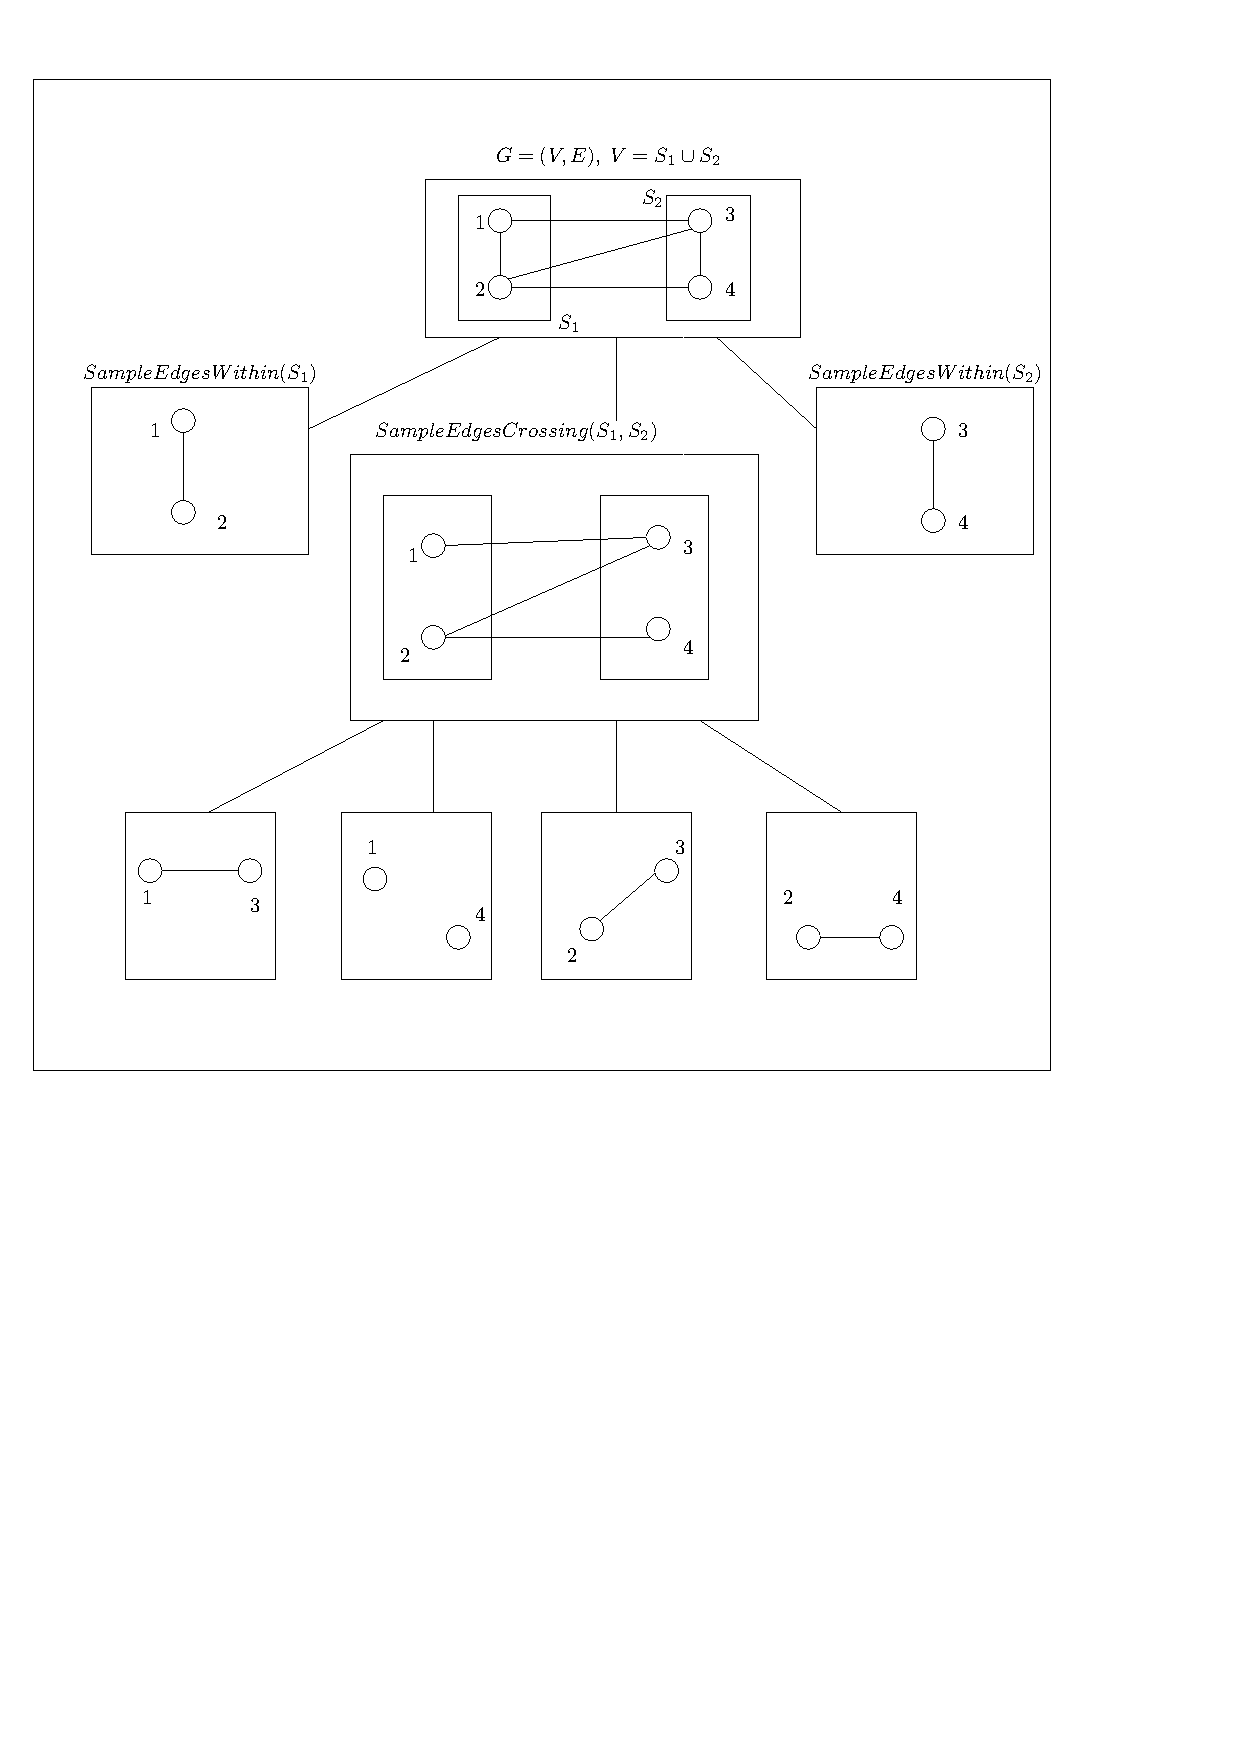
\includegraphics[scale=0.5]{alg-tree}
 
\end{figure}
\end{frame}

\begin{frame}
 \frametitle{Running Time}

 
 $f(n)$ := running time of $SampleEdgesWithin(S)$
 
 \leavevmode\hphantom{ }
 \leavevmode\hphantom{ }
 
 $g(n)$ := running time of $SampleEdgesCrossing(S, R)$
 
 \leavevmode\hphantom{ }
 \leavevmode\hphantom{ }
 
 where $n = |R| = |S|$
 
 $$ g(n) = 4 \ g(n/2) + \mathcal{O}(n^\omega) $$
 $$ f(n) = 2 \ f(n/2) + g(n) + \mathcal{O}(n^\omega) $$
 
  \leavevmode\hphantom{ }
 \leavevmode\hphantom{ }
 
 By master theorem the final running time is $\mathcal{O}(n^\omega)$
 
\end{frame}




%------------------------------------------------


%------------------------------------------------
\section{Conclusion}
%------------------------------------------------

\begin{frame}
 \frametitle{Other algorithms}
 
 \large\textbf{Determinant Based}
 \begin{itemize}
  \item \cite{COLBOURN1989271} uses a similar 6 way divide and conquer approach, but handles update using gaussian elimination. Runs in $\mathcal{O}(N^3)$
  \item \cite{COLBOURN1996268} improves the previous algorithm to $\mathcal{O}(N^\omega)$ using a modification of LU decomposition.
 \end{itemize}

 
 \large\textbf{Approximation Algorithms}
 \begin{itemize}
  \item \cite{10.5555/1747597.1748019} built upon the Aldous-Broder algorithm by using the fast approximate laplacian solver of \cite{10.1145/1007352.1007372} to shortcut already visited regions
 \end{itemize}

 
\end{frame}

\begin{frame}{Initial Motivation and Future work }
 
 \begin{itemize}
  \item Motivated by problem of efficiently sampling uniform spanning trees for dynamic graphs
 \item Recently \cite{DBLP:journals/corr/abs-2004-12739} also used the same identity for showing that \textbf{REACHABILITY} problem is in \texttt{DynFO} + \texttt{Mod} $2(\leq, +, \times)$. Hence we explored the possibility of using the same framework for sampling spanning trees in the dynamic setting.
 
 \end{itemize}


 
 
 
\end{frame}


%------------------------------------------------

%------------------------------------------------


% white!50!red
% white!50!green

%------------------------------------------------

\begin{frame}
 \frametitle{Three Takeaways \footnote{\url{https://math.stanford.edu/~vakil/threethings.html}}}
 
 \begin{enumerate}
  \item \textbf{Random Spanning Trees} 
  \item \textbf{Electric Networks}
  \item \textbf{Sherman-Morrison-Woodbury Identity}
 \end{enumerate}

 
 
\end{frame}



\begin{frame}
\centering
\Huge{Thank You}
\begin{figure}
 \centering
 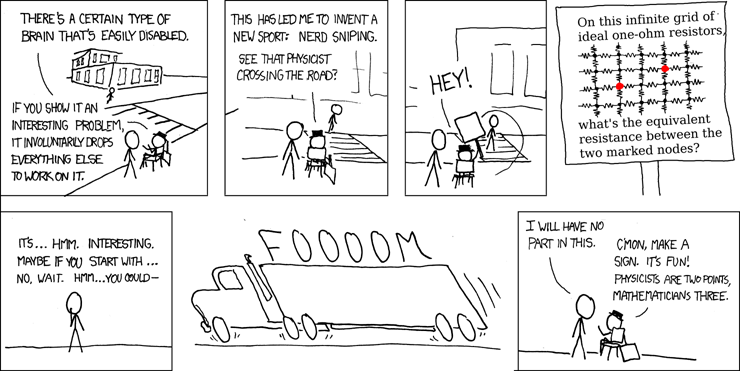
\includegraphics[scale=0.4]{nerd_sniping.png}
 \caption{Obligatory xkcd \footnote{\url{https://xkcd.com/356/}} }
\end{figure}



\end{frame}

% 
% \begin{frame}
% \frametitle{References}
% \footnotesize{
% \begin{thebibliography}{99} % Beamer does not support BibTeX so references must be inserted manually as below
% \bibitem[Smith, 2012]{p1} John Smith (2012)
% \newblock Title of the publication
% \newblock \emph{Journal Name} 12(3), 45 -- 678.
% \end{thebibliography}
% }
% \end{frame}

\begin{frame}[allowframebreaks]
\frametitle{References}
\Fontvi
% \lipsum[1]
 \bibliographystyle{amsalpha}
\bibliography{/home/bhishma/Documents/code/masters-thesis/thesis/example.bib}
\end{frame}


%------------------------------------------------

%----------------------------------------------------------------------------------------

\end{document} 
